%!TEX root = ../template.tex
%%%%%%%%%%%%%%%%%%%%%%%%%%%%%%%%%%%%%%%%%%%%%%%%%%%%%%%%%%%%%%%%%%%%
%% dmem_validation.tex
%% NOVA thesis document file
%%%%%%%%%%%%%%%%%%%%%%%%%%%%%%%%%%%%%%%%%%%%%%%%%%%%%%%%%%%%%%%%%%%%

\typeout{NT FILE dmem_validation.tex}

\chapter{Validation of the DMEM Strategy for Masonry Arch Bridges}
\label{cha:dmem-validation}

This chapter validates the \gls{DMEM} modelling strategy described in \Cref{cha:dmem-strategy}. The validation is based on the extensive experimental campaign carried out at the Bolton Institute on large-scale brickwork masonry arch bridge prototypes \cite{Melbourne1995,Melbourne1997}. The campaign includes single- and multi-span bridges, attached and detached spandrel walls, and multi-ring arch barrels with and without ring separation. These tests have become a reference benchmark for numerical modelling strategies because they involve realistic component interaction, nonlinear response, and clearly identifiable collapse mechanisms.

The material in this chapter is based on the journal article published by the author and co-workers \cite{Bonatte2026DMEM}. Here, the results are rewritten as thesis content and interpreted in relation to the modelling strategy that will support the remaining PhD research. The objective is not only to verify peak load predictions, but also to assess whether the numerical model can reproduce the load-displacement response, damage evolution, influence of defects, and three-dimensional interaction between arch barrels, backfill, and spandrel walls.

\section{Experimental Campaign}
\label{sec:bolton-campaign}

The Bolton Institute experimental campaign tested large-scale multi-ring brickwork bridge specimens under monotonic vertical line loads applied at deck level. The bridges were constructed with engineering bricks and mortar, with backfill placed above the arch barrel. Loads were applied through a rigid steel beam resting on the backfill surface, so the applied force was distributed across the bridge width before reaching the arch barrel. Instrumentation included displacement transducers, strain gauges, and soil pressure cells, allowing the global load-displacement response, crack development, and backfill pressure mobilisation to be monitored \cite{Melbourne1995,Melbourne1997}.

\begin{figure}[htbp]
\centering
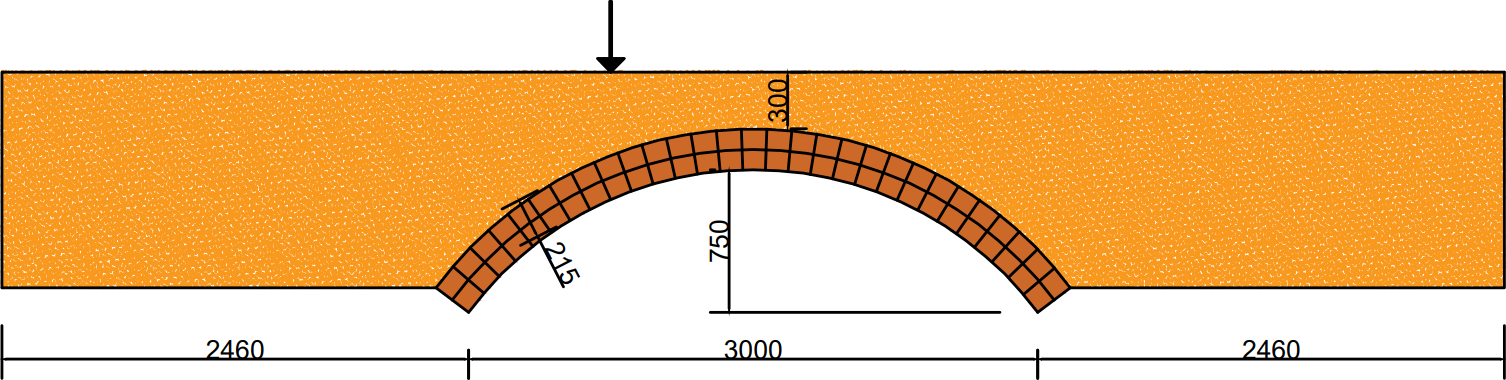
\includegraphics[width=0.95\linewidth]{./Figures/image6.png}
\caption{Geometry of representative Bolton bridge specimens: single-span Bridge 3.1 \cite{Melbourne1995}.}
\label{fig:bolton-bridge-31-geometry}
\end{figure}

\begin{figure}[htbp]
\centering
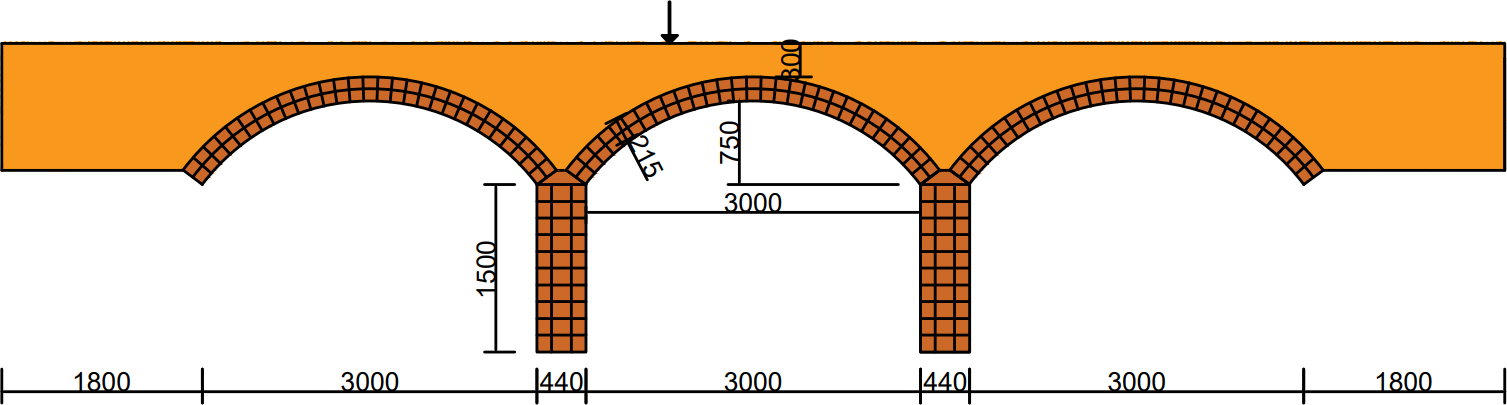
\includegraphics[width=0.95\linewidth]{./Figures/image7.png}
\caption{Geometry of representative Bolton bridge specimens: multi-span Bridge MS2 \cite{Melbourne1997}.}
\label{fig:bolton-ms2-geometry}
\end{figure}

Six single-span specimens and three multi-span specimens are considered in the validation. The single-span group includes 3 m and 5 m span bridges, bridges with detached spandrel walls, bridges with attached spandrel walls, and bridges with ring separation defects. The multi-span group includes three-span bridges with 3 m spans and different spandrel-wall and loading configurations.

\begin{table}[htbp]
\centering
\small
\setlength{\tabcolsep}{3pt}
\caption{Geometric characteristics and experimental failure loads of the Bolton bridge specimens \cite{Melbourne1995,Melbourne1997}.}
\label{tab:bolton-geometry}
\resizebox{\textwidth}{!}{%
\begin{tabular}{ccccclc}
\hline
Bridge & Span (m) & Width (m) & Rings & Defects & Load configuration & $F_\mathrm{exp}$ (kN)\\
\hline
3.1 & 3 & 2.88 & 2 & Detached spandrels & Quarter span & 540\\
3.2 & 3 & 2.88 & 2 & Detached spandrels; ring separation & Quarter span & 360\\
3.3 & 3 & 3.54 & 2 & None & Quarter span & 600\\
3.4 & 3 & 3.54 & 2 & Ring separation & Quarter span & 320\\
5.1 & 5 & 3.01 & 4 & Detached spandrels & Quarter span & 1720\\
5.2 & 5 & 3.01 & 4 & Detached spandrels; ring separation & Quarter span & 500\\
MS1 & $3\times3$ & 3.54 & 2 & None & Quarter span of central arch & 455\\
MS2 & $3\times3$ & 2.88 & 2 & Detached spandrels & Quarter span of central arch & 320\\
MS3 & $3\times3$ & 2.54 & 2 & None & 240 mm north of crown & 325\\
\hline
\end{tabular}
}
\end{table}

All 3 m single-span specimens were segmental circular arches with two arch rings and an arch thickness of 215 mm. The 5 m specimens included four arch rings. Ring separation was introduced by weakening the interface between adjacent rings, so that the individual rings could slide and deform more independently. This defect is especially relevant for existing bridges because loss of composite action between rings can substantially reduce load-carrying capacity.

\section{Material Properties}
\label{sec:bolton-materials}

The original campaign included material and component tests on brickwork and backfill. Brickwork properties were obtained from compression tests, shear tests on small panels, and measurements of unit weight. Backfill properties were obtained from shear-box tests and density measurements. Some parameters required by the \gls{DMEM} formulation were not available directly, namely Poisson's ratio, tensile strength, and fracture energies. These values were therefore taken from or aligned with previous numerical validations of the same experiments \cite{Zhang2018,Tubaldi2020a,Zizi2024}.

\begin{table}[htbp]
\centering
\caption{Material parameters with constant values adopted in the validation models \cite{Bonatte2026DMEM}.}
\label{tab:dmem-constant-materials}
\begin{tabular}{lccccccc}
\hline
Material & $\gamma$ (kN/m$^3$) & $\nu$ (-) & $\Phi$ (-) & $c$ (MPa) & $f_t$ (MPa) & $G_t$ (kN/m) & $G_c$ (kN/m)\\
\hline
Masonry & -- & 0.15 & -- & 0.29 & 0.20 & 0.02 & 3.00\\
Backfill & 22.2 & 0.20 & 1.47 & 0.001 & 0.001 & 0.01 & --\\
\hline
\end{tabular}
\end{table}

\begin{table}[htbp]
\centering
\caption{Bridge-dependent material parameters adopted in the validation models \cite{Bonatte2026DMEM}.}
\label{tab:dmem-variable-materials}
\begin{tabular}{lccccc}
\hline
Bridge & $\gamma_m$ (kN/m$^3$) & $E_m$ (GPa) & $f_{cm}$ (MPa) & $\Phi_m$ (-) & $E_b$ (GPa)\\
\hline
3.1 & 22.7 & 15.9 & 26.5 & 0.64 & 0.20\\
3.2 & 22.7 & 15.9 & 26.5 & 0.64 & 0.20\\
3.3 & 22.7 & 15.9 & 26.5 & 0.50 & 0.20\\
3.4 & 22.7 & 15.9 & 26.5 & 0.50 & 0.20\\
5.1 & 22.7 & 9.2 & 18.1 & 0.64 & 0.20\\
5.2 & 22.7 & 25.0 & 28.2 & 0.64 & 0.20\\
MS1 & 22.4 & 16.2 & 26.8 & 0.50 & 0.05\\
MS2 & 22.4 & 16.2 & 26.8 & 0.50 & 0.05\\
MS3 & 22.4 & 22.3 & 27.7 & 0.50 & 0.05\\
\hline
\end{tabular}
\end{table}

For the backfill, the Young's modulus was adopted consistently with previous numerical studies. A value of 0.20 GPa was used for the single-span specimens and 0.05 GPa for the multi-span specimens, following the calibration choices available in the benchmark literature. A nominal cohesion was assigned to the backfill to improve numerical stability while keeping the material essentially frictional. Since the macro-element formulation does not include Poisson effects, the model cannot directly reproduce all confinement effects between backfill and spandrel walls. This limitation is relevant when interpreting the stiffness of specimens with strong transverse restraint.

\section{Numerical Modelling Assumptions}
\label{sec:dmem-validation-modelling}

The numerical models were developed in HiStrA Bridges \cite{HiStrA2022}. Two modelling approaches were used. For bridges with detached spandrel walls and symmetric line loading, a strip model was adopted. This model includes one set of elements across the width of the arch and backfill and is computationally efficient for square bridges under uniformly distributed transverse line loads. For bridges with attached spandrel walls, a full three-dimensional model was required, with several macro-elements across the bridge width to represent transverse interaction between the arch barrel, backfill, load print, and spandrel walls.

\begin{figure}[htbp]
\centering
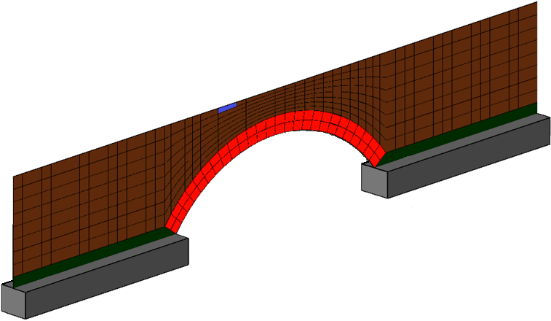
\includegraphics[width=0.8\linewidth]{./Figures/image8.png}
\caption{Strip-model representation for bridges with detached spandrel walls.}
\label{fig:dmem-strip-model}
\end{figure}

\begin{figure}[htbp]
\centering
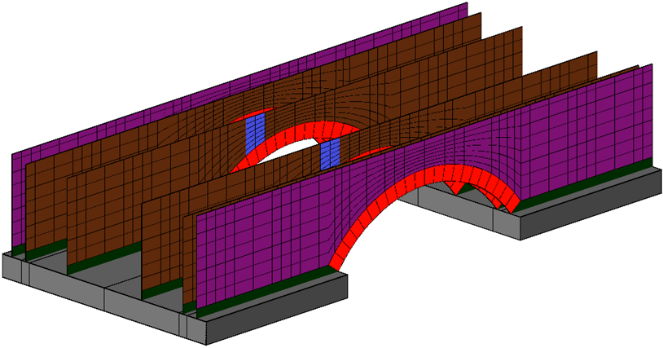
\includegraphics[width=0.8\linewidth]{./Figures/image10.png}
\caption{Three-dimensional model used for bridges with attached spandrel walls.}
\label{fig:dmem-3d-model}
\end{figure}

\begin{figure}[htbp]
\centering
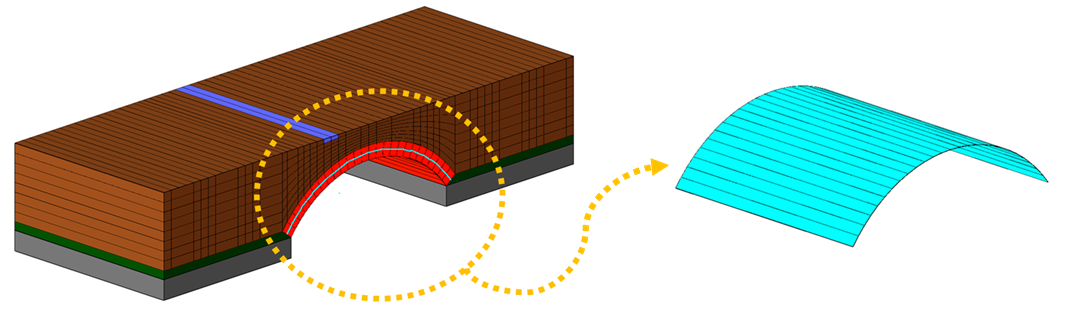
\includegraphics[width=0.8\linewidth]{./Figures/image12.png}
\caption{Zero-thickness weak interfaces introduced to represent ring separation between arch rings.}
\label{fig:dmem-ring-separation}
\end{figure}

The nonlinear constitutive response was assigned according to the failure mechanism represented by each link. Flexural failure was modelled with linear softening in tension and compression, diagonal shear was modelled with an elasto-plastic law and fixed ductility, and sliding was governed by an elasto-plastic Mohr--Coulomb law. For ring separation, weak frictional interfaces were inserted between arch rings using the friction value reported for the damp-sand defective interface in the experimental campaign.

The analyses were performed with a nonlinear incremental Newton--Raphson scheme and an energy convergence criterion. Arc-length control was used to regulate the load increment and improve convergence around peak and post-peak response. Most models used macro-elements smaller than 30 cm and interface spring spacing below approximately 10 cm. Refined meshes were introduced in selected models to study mesh sensitivity and to better represent ring-separation behaviour.

\section{Single-Span Bridges}
\label{sec:dmem-single-span}

\subsection{Bridge 3.1: Detached Spandrel Walls}
\label{sec:dmem-bridge31}

Bridge 3.1 is a 3 m-span bridge with detached spandrel walls and no ring-separation defect. Two numerical meshes were considered. The coarse mesh used one macro-element through the arch thickness and 12 elements along the arch barrel, with a characteristic size of approximately 30 cm. The refined mesh used two macro-elements through the arch thickness and 26 elements along the arch barrel, allowing the two-ring construction to be represented in greater detail.

\begin{figure}[htbp]
\centering
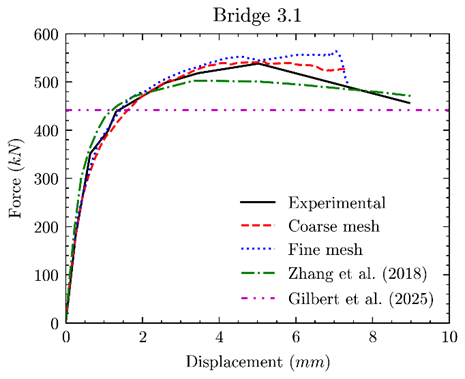
\includegraphics[width=0.85\linewidth]{./Figures/image13.png}
\caption{Experimental and numerical load-displacement response for Bridge 3.1.}
\label{fig:bridge31-load-displacement}
\end{figure}

\begin{figure}[htbp]
\centering
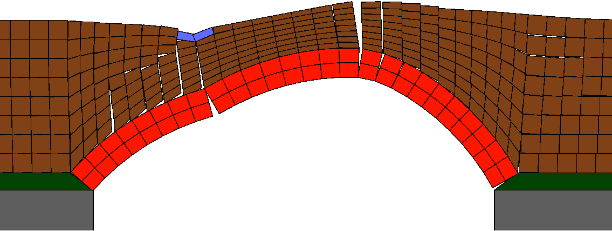
\includegraphics[width=0.8\linewidth]{./Figures/image15.png}
\caption{Predicted collapse mechanism for Bridge 3.1.}
\label{fig:bridge31-collapse}
\end{figure}

The numerical response agrees well with the experimental curve in terms of initial stiffness, peak load, and post-peak trend. The refined and coarse meshes provide similar global responses, indicating a low mesh sensitivity for this case. This is important because it shows that the \gls{DMEM} can avoid strong localisation dependence even when softening material laws are used. The predicted collapse mechanism also agrees with the experimental evidence and with previous mesoscale simulations \cite{Zhang2018}. The coarse and refined analyses required only seconds to complete on standard hardware, confirming the low computational cost of the method.

The stress and damage fields indicate the formation of four radial cracks in the arch barrel. The stress distribution across the two rings remains essentially continuous, showing that the rings behave collaboratively when no ring-separation defect is present. The backfill also contributes to the response by diffusing the applied line load and by providing passive resistance as the arch deforms upward near the extrados.

\begin{figure}[htbp]
\centering
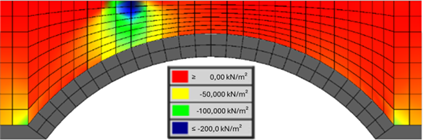
\includegraphics[width=0.8\linewidth]{./Figures/image18.png}
\caption{Principal compressive stress field in the backfill of Bridge 3.1 at a low load level.}
\label{fig:bridge31-backfill-low}
\end{figure}

\begin{figure}[htbp]
\centering
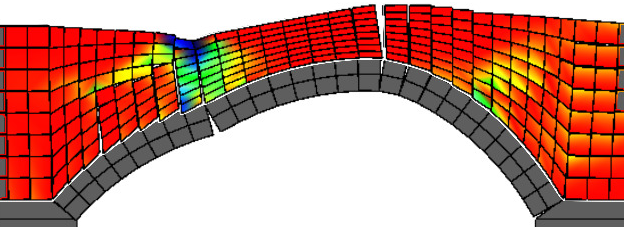
\includegraphics[width=0.8\linewidth]{./Figures/image23.png}
\caption{Principal compressive stress field in the backfill of Bridge 3.1 near peak load, showing passive resistance mobilisation.}
\label{fig:bridge31-backfill-peak}
\end{figure}

\subsection{Bridge 5.1: Detached Spandrel Walls}
\label{sec:dmem-bridge51}

Bridge 5.1 is a 5 m-span bridge with detached spandrel walls and four arch rings. The first strip model reproduced the peak load satisfactorily but underestimated the experimental stiffness. The discrepancy is linked to the experimental observation that the detached spandrel and wing walls interacted with the backfill more strongly than expected. This interaction increased the measured stiffness and even caused visible cracking at the base of the spandrel walls during the test.

\begin{figure}[htbp]
\centering
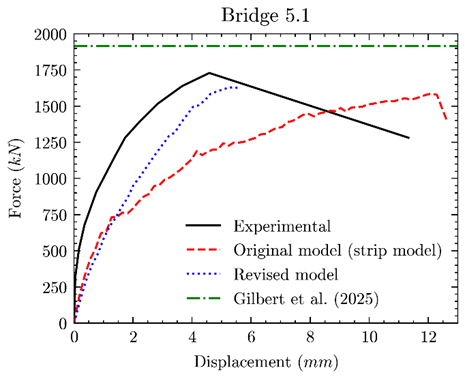
\includegraphics[width=0.85\linewidth]{./Figures/image24.png}
\caption{Experimental and numerical load-displacement response for Bridge 5.1.}
\label{fig:bridge51-load-displacement}
\end{figure}

To represent this effect, a revised model explicitly included the detached spandrel walls connected to the backfill but not to the arch barrel. This improved the agreement with the experimental response, although the measured stiffness remained higher than the numerical prediction. The remaining discrepancy is consistent with the current limitation of the macro-element formulation regarding Poisson confinement effects. The result shows that detached spandrel walls may not always be ignored, even when no mechanical connection to the arch barrel exists, because frictional interaction with the backfill can influence the global stiffness.

\subsection{Bridge 3.2: Detached Spandrel Walls and Ring Separation}
\label{sec:dmem-bridge32}

Bridge 3.2 has the same nominal geometry as Bridge 3.1, but includes a ring-separation defect. The defect was represented in the numerical model by a weak frictional interface between the two arch rings.

\begin{figure}[htbp]
\centering
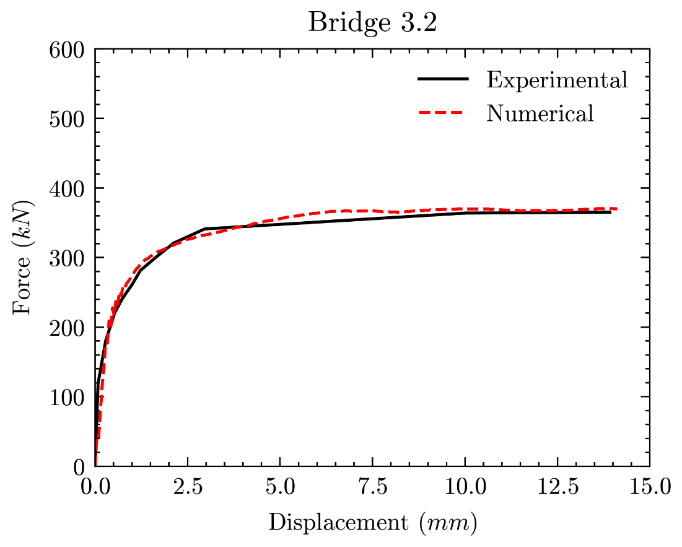
\includegraphics[width=0.85\linewidth]{./Figures/image26.png}
\caption{Experimental and numerical load-displacement response for Bridge 3.2.}
\label{fig:bridge32-load-displacement}
\end{figure}

\begin{figure}[htbp]
\centering
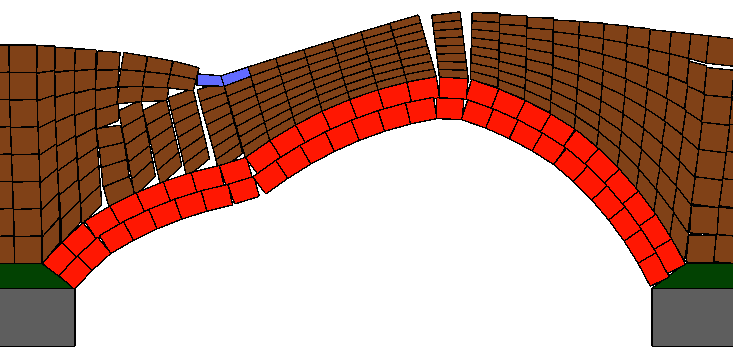
\includegraphics[width=0.8\linewidth]{./Figures/image28.png}
\caption{Predicted collapse mechanism for Bridge 3.2.}
\label{fig:bridge32-collapse}
\end{figure}

The \gls{DMEM} model reproduces the experimental response very closely. The peak load is reduced from approximately 540 kN in Bridge 3.1 to approximately 360 kN in Bridge 3.2, showing the strong influence of ring separation on the load-carrying capacity. The stress distribution also changes substantially. In Bridge 3.1, the two rings act nearly monolithically; in Bridge 3.2, stress discontinuities appear at the defective interface and the individual rings develop more independent compression and tension zones. This confirms that the weak-interface modelling strategy is able to capture the mechanical effect of ring separation.

\subsection{Bridge 5.2: Detached Spandrel Walls and Ring Separation}
\label{sec:dmem-bridge52}

Bridge 5.2 is the defective counterpart of Bridge 5.1 and includes ring separation between four arch rings. The \gls{DMEM} prediction again matches the experimental response well, including the peak load and collapse pattern.

\begin{figure}[htbp]
\centering
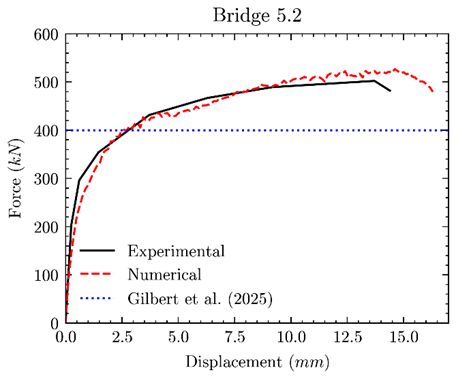
\includegraphics[width=0.85\linewidth]{./Figures/image31.png}
\caption{Experimental and numerical load-displacement response for Bridge 5.2.}
\label{fig:bridge52-load-displacement}
\end{figure}

\begin{figure}[htbp]
\centering
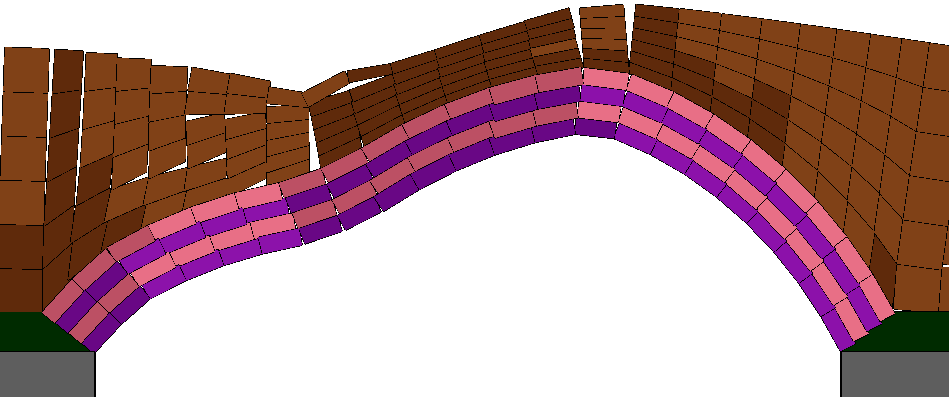
\includegraphics[width=0.8\linewidth]{./Figures/image33.png}
\caption{Stress distribution in the defective arch barrel of Bridge 5.2.}
\label{fig:bridge52-stress}
\end{figure}

The capacity reduction caused by ring separation is much larger for the 5 m bridge than for the 3 m bridge. Bridge 5.1 reached approximately 1720 kN, whereas Bridge 5.2 reached approximately 500 kN, corresponding to a reduction of about 71\%. This reduction is larger than the reduction between Bridges 3.1 and 3.2 because the 5 m bridge contains more defective ring interfaces. The comparison confirms that multi-ring interaction is a dominant mechanism in the structural response of these specimens.

\subsection{Bridge 3.3: Attached Spandrel Walls}
\label{sec:dmem-bridge33}

Bridge 3.3 is a 3 m-span bridge with attached spandrel walls and no ring separation. This configuration requires a three-dimensional model because the spandrel walls interact with the arch barrel and backfill, producing transverse effects that cannot be represented by a strip model.

\begin{figure}[htbp]
\centering
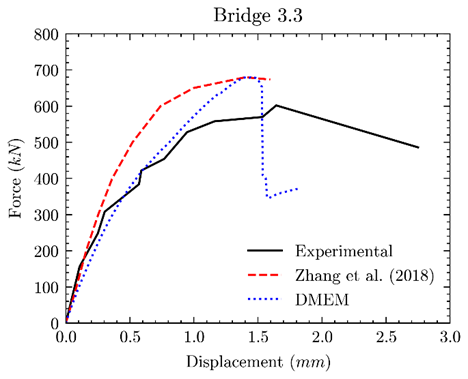
\includegraphics[width=0.85\linewidth]{./Figures/image35.png}
\caption{Experimental and numerical load-displacement response for Bridge 3.3.}
\label{fig:bridge33-load-displacement}
\end{figure}

\begin{figure}[htbp]
\centering
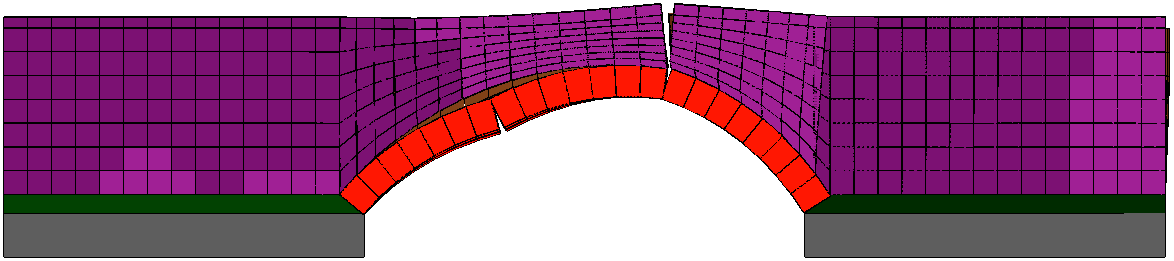
\includegraphics[width=0.75\linewidth]{./Figures/image37.png}
\caption{Predicted collapse mechanism for Bridge 3.3 with attached spandrel walls.}
\label{fig:bridge33-collapse}
\end{figure}

The numerical model captures the higher stiffness and greater load capacity associated with the attached spandrel walls. Compared with the detached-spandrel specimen Bridge 3.1, the attached-spandrel configuration produces a significant increase in peak load. Some discrepancy remains between the numerical and experimental capacities. This may be related to cracking observed experimentally between the arch barrel extrados and the attached spandrel walls at relatively low load levels, before the main arch-barrel hinge mechanism developed.

\begin{figure}[htbp]
\centering
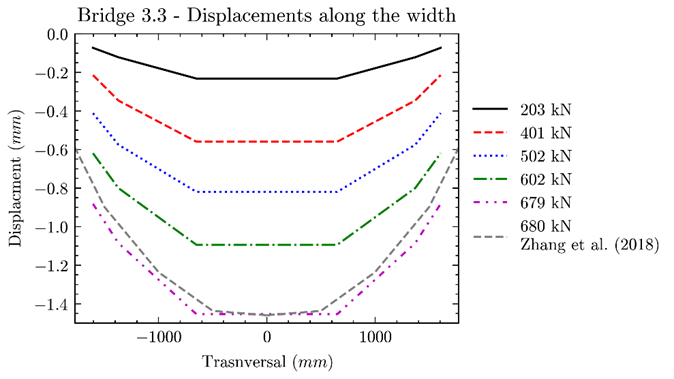
\includegraphics[width=0.8\linewidth]{./Figures/image39.png}
\caption{Transverse displacement distribution along the arch width for Bridge 3.3.}
\label{fig:bridge33-width-displacements}
\end{figure}

The transverse displacement profile confirms the need for three-dimensional modelling. As the load increases, displacements near the spandrel walls remain smaller than those near the centre of the arch barrel. The central part of the arch therefore carries a different deformation demand from the edge zones, and the bridge response cannot be represented by an effective-width assumption alone when attached spandrel walls are mechanically active.

\subsection{Bridge 3.4: Attached Spandrel Walls and Ring Separation}
\label{sec:dmem-bridge34}

Bridge 3.4 combines attached spandrel walls with ring separation. The numerical model follows the Bridge 3.3 modelling strategy but introduces the weak frictional interface between arch rings.

\begin{figure}[htbp]
\centering
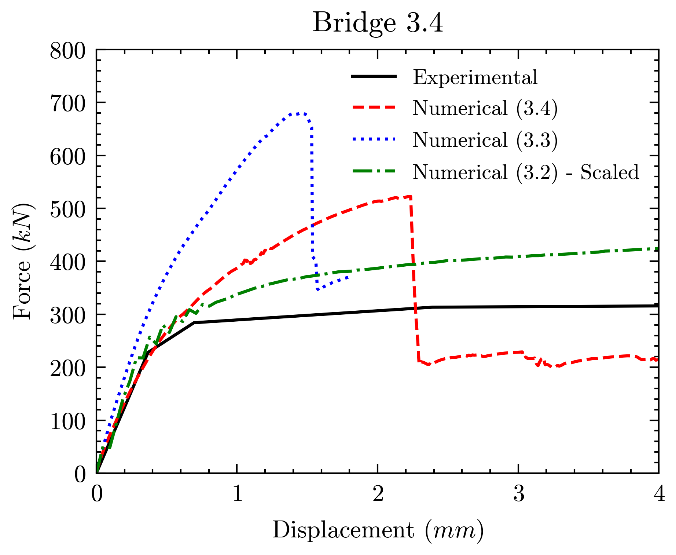
\includegraphics[width=0.85\linewidth]{./Figures/image40.png}
\caption{Experimental and numerical load-displacement response for Bridge 3.4, including comparison with related configurations.}
\label{fig:bridge34-load-displacement}
\end{figure}

\begin{figure}[htbp]
\centering
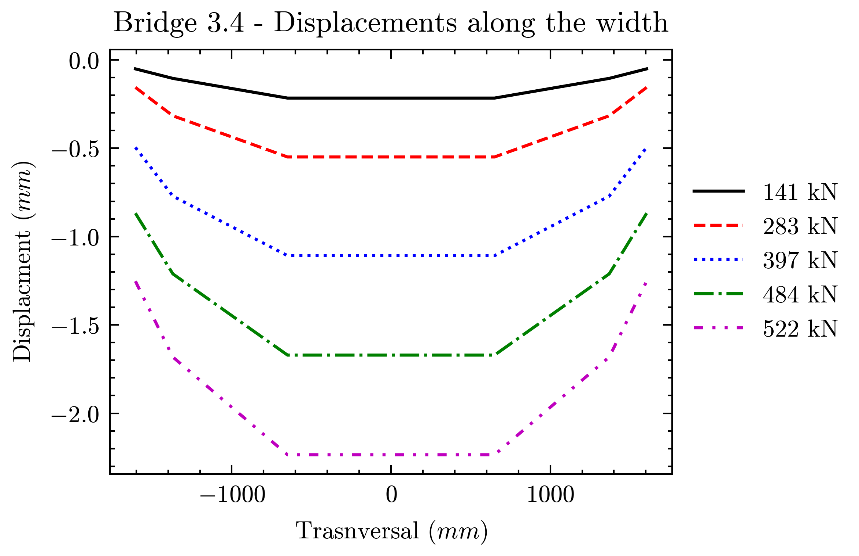
\includegraphics[width=0.8\linewidth]{./Figures/image43.png}
\caption{Transverse displacement distribution along the arch width for Bridge 3.4.}
\label{fig:bridge34-width-displacements}
\end{figure}

The experimental peak load of Bridge 3.4 was lower than might be expected from the presence of attached spandrel walls. The campaign reported early cracking between the arch barrel and the spandrel walls, which likely reduced the effective composite action. The numerical response falls between the defective detached-spandrel bridge and the undamaged attached-spandrel bridge, which is mechanically consistent. Relative to Bridge 3.3, the ring separation reduces the numerical capacity by approximately 23\%. The transverse displacement profile again shows smaller displacements near the spandrel walls and larger displacements at mid-width.

\section{Multi-Span Bridges}
\label{sec:dmem-multi-span}

The multi-span specimens provide a more demanding validation because they involve pier movement, interaction between adjacent spans, and different load paths. The three analysed specimens have three spans of 3 m each. Bridge MS2 has detached spandrel walls, while Bridges MS1 and MS3 have attached spandrel walls. Since no ring-separation defect was introduced in the multi-span tests, the arch barrel was modelled with a single layer in the numerical simulations.

\subsection{Bridge MS2: Detached Spandrel Walls}
\label{sec:dmem-ms2}

Bridge MS2 was modelled using the strip approach, consistent with the detached-spandrel single-span bridges. The numerical model reproduces both the arch load-displacement response and the horizontal displacement response of the piers.

\begin{figure}[htbp]
\centering
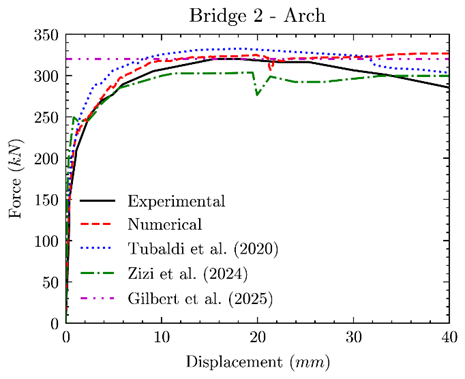
\includegraphics[width=0.85\linewidth]{./Figures/image44.png}
\caption{Arch load-displacement response for Bridge MS2.}
\label{fig:ms2-arch-response}
\end{figure}

\begin{figure}[htbp]
\centering
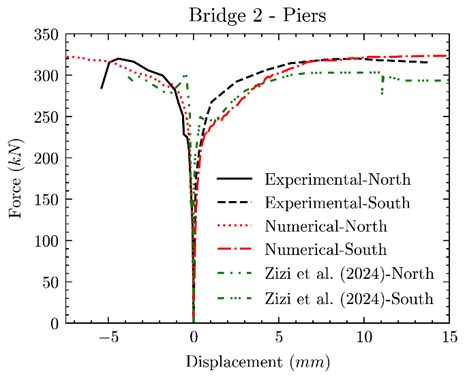
\includegraphics[width=0.85\linewidth]{./Figures/image45.png}
\caption{Pier displacement response for Bridge MS2.}
\label{fig:ms2-pier-response}
\end{figure}

\begin{figure}[htbp]
\centering
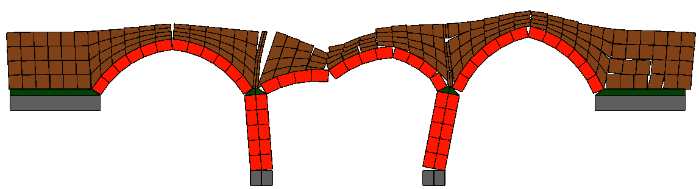
\includegraphics[width=0.85\linewidth]{./Figures/image47.png}
\caption{Predicted collapse mechanism for Bridge MS2.}
\label{fig:ms2-collapse}
\end{figure}

The agreement with the experiment is good in terms of initial stiffness, peak load, and post-peak response. The predicted collapse mechanism is also consistent with the observed damage pattern and with previous numerical studies \cite{Tubaldi2020a,Zizi2024}. The model shows that the \gls{DMEM} strategy can reproduce not only local arch-barrel failure but also the global mechanism involving pier displacement and interaction between spans.

\subsection{Bridges MS1 and MS3: Attached Spandrel Walls}
\label{sec:dmem-ms1-ms3}

Bridge MS1 includes attached spandrel walls and was loaded at the quarter span of the central arch. The experimental campaign reported significant discrepancies between two load-cell readings, so the measured failure load should be interpreted with caution. Nevertheless, the initial load-displacement response is reproduced satisfactorily by the model, indicating that the stiffness of the bridge in the early nonlinear range is captured.

\begin{figure}[htbp]
\centering
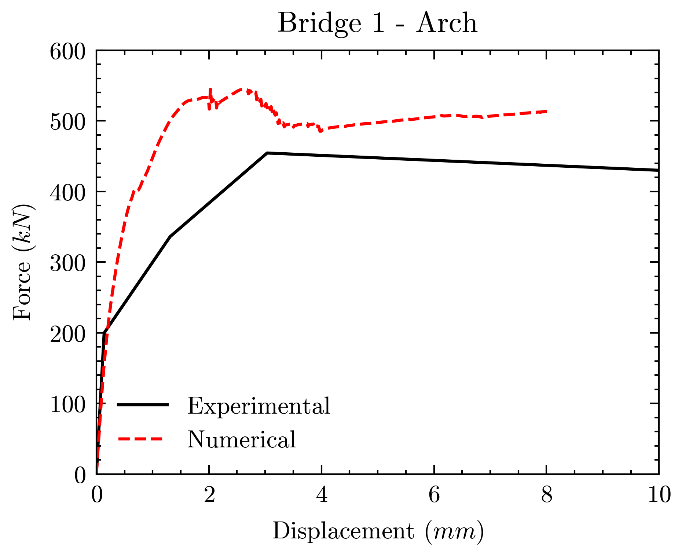
\includegraphics[width=0.8\linewidth]{./Figures/image50.png}
\caption{Pier load-displacement response for Bridge MS1.}
\label{fig:ms1-response}
\end{figure}

Bridge MS3 was subjected to a different loading arrangement. The vertical load was applied 240 mm north of the crown of the central span, and additional concrete blocks with a total weight of 48 kN were placed on the northern span to modify the failure mechanism. The numerical simulation therefore used three stages: self-weight, added block weight, and increasing vertical load.

\begin{figure}[htbp]
\centering
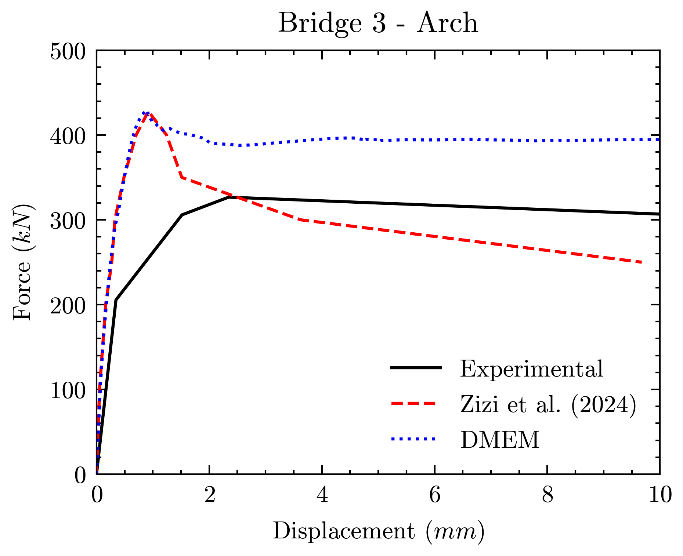
\includegraphics[width=0.8\linewidth]{./Figures/image51.png}
\caption{Load-displacement response for Bridge MS3.}
\label{fig:ms3-response}
\end{figure}

\begin{figure}[htbp]
\centering
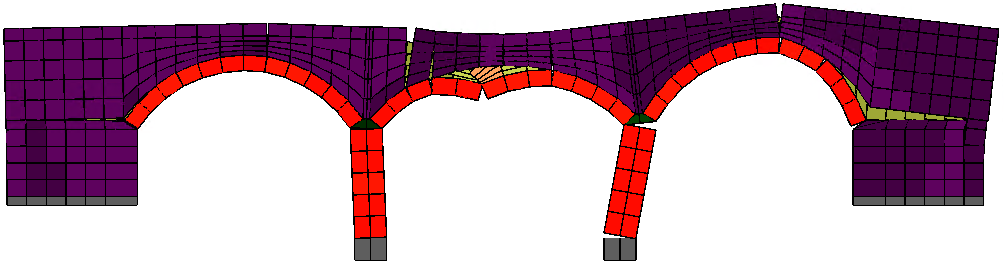
\includegraphics[width=0.85\linewidth]{./Figures/image53.png}
\caption{Predicted damage and collapse pattern for Bridge MS3.}
\label{fig:ms3-collapse}
\end{figure}

The \gls{DMEM} and previous \gls{FEM} predictions agree well up to peak load. Differences appear in the post-peak response, where the \gls{FEM} result shows a sharper drop and the \gls{DMEM} response exhibits more gradual plastic deformation. This discrepancy is not unexpected because the experimental material data do not define post-peak masonry properties completely. The agreement in failure mechanism is more relevant for the thesis framework, as it confirms that the model captures the governing load path and damage localisation.

\section{Discussion of Validation Results}
\label{sec:dmem-validation-discussion}

The validation campaign demonstrates that the \gls{DMEM} strategy is able to reproduce the main structural behaviours observed in the Bolton tests. For bridges with detached spandrel walls, efficient strip models provide accurate predictions of peak load, load-displacement response, and collapse mechanism. For bridges with attached spandrel walls, three-dimensional models are necessary and successfully reproduce the transverse displacement gradients caused by wall restraint.

The influence of ring separation is captured with particular clarity. In both 3 m and 5 m single-span bridges, weak interfaces between arch rings reduce composite action, produce discontinuous stress distributions across the rings, and substantially reduce load capacity. The effect is especially severe in Bridge 5.2 because multiple defective interfaces are present. This confirms that ring separation should be represented explicitly when assessing existing multi-ring masonry arch bridges.

The backfill is also shown to be a governing component. It diffuses the vertical line load and provides passive resistance where the arch barrel uplifts. These effects emerge naturally from the explicit backfill model rather than from empirical distribution rules. The limitation is that the current macro-element formulation does not include Poisson confinement effects, which affects stiffness predictions when spandrel walls strongly confine the backfill.

From a computational viewpoint, the method is appropriate for the remaining PhD work. Even the three-dimensional models with attached spandrel walls and weak interfaces run in minutes rather than hours or days. This makes the method compatible with sensitivity studies, uncertainty propagation, and the future development of fragility or resilience indicators.

\section{Chapter Conclusions}
\label{sec:dmem-validation-conclusions}

The validation presented in this chapter supports the use of the \gls{DMEM} as the core structural modelling strategy in this thesis. The method predicts the load-carrying capacity of single- and multi-span masonry arch bridge specimens with accuracy comparable to more computationally expensive numerical strategies. It also reproduces the main failure mechanisms, including four-hinge arch mechanisms, pier-displacement mechanisms, ring separation effects, and transverse displacement profiles in bridges with attached spandrel walls.

The results show that the extension of the macro-element to interfaces on all six faces is essential for bridge applications. It enables explicit modelling of backfill load diffusion, passive resistance, and interaction with spandrel walls. The validation also identifies limitations that must be considered in subsequent applications, especially the absence of Poisson effects and the simplified constitutive representation of backfill.

For the PhD framework, the main conclusion is that the selected modelling strategy is sufficiently accurate and efficient to support broader analyses of masonry arch bridges under traffic, foundation-related actions, and flood-induced effects. The next stages of the thesis can therefore use the \gls{DMEM} model as a validated numerical engine for parametric, probabilistic, and decision-support developments.
